\section{Numeri complessi}

Se consideriamo l'insieme dei numeri reali $\R$ e i polinomi a coefficienti reali $\R[x]$ notiamo che non tutti i polinomi sono fattorizzabili \emph{completamente}: alcuni polinomi di grado $2$, in particolare quelli con discriminante negativo, non ammettono fattorizzazione in polinomi di grado $1$. Lo scopo dei numeri complessi è quindi quello di permettere la risoluzione di equazioni di secondo grado con delta negativo.

La più semplice equazione di secondo grado senza soluzioni in $\R$ è \[
    x^2 + 1 = 0.  
\] Infatti essa è equivalente a $x^2 = -1$, e siccome il quadrato di ogni numero reale è non negativo, nessun $x \in \R$ può soddisfarla. Si introduce per questo l'\emph{unità immaginaria} $i$.

\begin{definition}
    [Unità immaginaria] \label{def:immaginary_unit}
    Si dice \emph{unità immaginaria} il numero $i$ tale che \begin{equation}
        i^2 \deq -1.
    \end{equation}
\end{definition}

\begin{definition}
    [Insieme dei numeri complessi]
    Si dice \emph{insieme dei numeri complessi} l'insieme $C$ tale che \begin{equation}
        \C \deq \set{a + ib \suchthat a, b \in \R, i^2 = -1}.
    \end{equation}
\end{definition}

Un numero complesso $z$ può dunque essere pensato come una coppia di numeri reali: il primo viene detto \emph{parte reale di $z$}, e lo si indica con $\Re z$; il secondo viene detto \emph{parte immaginaria di $z$}, e lo si indica con $\Im z$.

Questa rappresentazione ci consente di rappresentare i numeri complessi come se fossero vettori nel piano (che viene quindi detto \emph{piano complesso}): la parte reale di un numero complesso è l'ascissa, la parte immaginaria è l'ordinata.

\begin{center}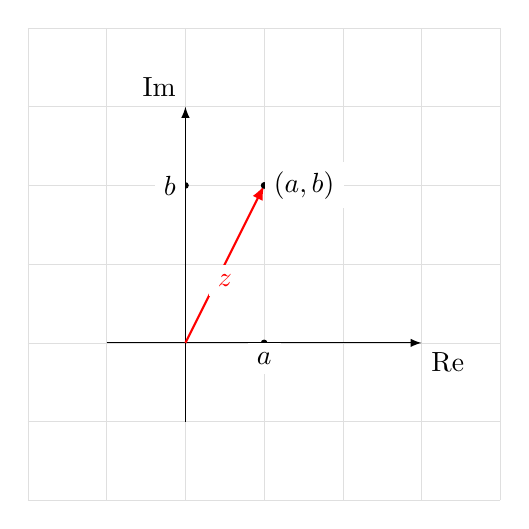
\begin{tikzpicture}[>=latex]
    \draw[step=1cm,gray!25!,very thin] (-2,-2) grid (4,4);
    \draw[thin,->] (-1,0) -- (3,0) node[anchor=north west] {Re};
    \draw[thin,->] (0,-1) -- (0,3) node[anchor=south east] {Im};
    \draw[red,thick,->] (0,0) coordinate (O) -- (1, 2)
    node[midway,below, fill=white] {$z$};
    \filldraw [black] (1,0) circle (1pt)
    node[below, fill=white] {$a$};
    \filldraw [black] (0,2) circle (1pt)
    node[left, fill=white] {$b$};
    \filldraw [black] (1,2) circle (1pt)
    node[right, fill=white] {$(a, b)$};
\end{tikzpicture}\end{center}

Avendo rappresentato i numeri complessi come vettori, viene spontaneo definire una quantità che rappresenti la \emph{lunghezza} del vettore.
\begin{definition}
    [Modulo di un numero complesso] Sia $z = a + ib \in \C$. Si dice \emph{modulo} di $z$ il numero reale \begin{equation}
        \abs*{z} \deq \sqrt{a^2 + b^2}. 
    \end{equation}
\end{definition}

Il modulo di $z$ è la lunghezza del vettore associato a $z$ per il teorema di Pitagora: il vettore è l'ipotenusa di un triangolo rettangolo che ha un cateto lungo $a$ e un cateto lungo $b$. Per questo l'unico numero complesso che ha modulo $0$ è il numero $0 +i0$.

Ovviamente due numeri complessi $z, w \in \C$ sono uguali se e solo se hanno la stessa parte reale e la stessa parte immaginaria, ovvero se e solo se rappresentano lo stesso vettore nel piano complesso.

Possiamo inoltre definire due operazioni sui numeri complessi: una somma \begin{equation}
    (a + ib) + (c + id) = (a + c) + i(b + d) \in \C
\end{equation} e un prodotto \begin{equation}
    (a + ib) \cdot (c + id) = ac + iad + ibc + i^2bd = (ac - bd) + i(ad + bc).
\end{equation} Notiamo che $i^2bd = -bd$ per definizione dell'unità immaginaria.

La somma è definita come una qualunque somma tra vettori: nel piano complesso la somma si effettua con il metodo del parallelogramma, oppure sommando tra di loro le componenti (ovvero la parte reale e la parte immaginaria). Il prodotto non sembra avere un significato concreto; tuttavia nel seguito riusciremo a far vedere come i prodotti tra numeri complessi corrispondono a \emph{rotazioni} dei vettori nel piano.

Le due operazioni di somma e prodotto soddisfano la proprietà commutativa, la proprietà associativa e la proprietà distributiva della somma rispetto al prodotto. Notiamo inoltre che il numero complesso $0 + i0$ è elemento neutro rispetto alla somma: \[
    (a + ib) + (0 + i0) = (a + 0) + i(b + 0) = a + ib,    
\] e il numero complesso $1 + i0$ è l'elemento neutro del prodotto: \[
    (a + ib) \cdot (1 + i0) = (a\cdot 1 - b\cdot 0) + i(a\cdot 0 + b\cdot 1) = a + ib.    
\] Inoltre, ogni numero complesso ha un opposto: infatti dato $z = a+ib \in \C$ il suo opposto è dato da $-z = -a-ib$. Infatti \[
    z + (-z) = (a+ib) + (-a-ib) = 0 + i0,
\] cioè l'elemento neutro della somma.

Prima di vedere se ogni numero ammette un \emph{inverso moltiplicativo}, ovvero un reciproco, introduciamo una nuova operazione sui numeri complessi.

\begin{definition}
    [Coniugato complesso]
    Sia $z \in \C$ un numero complesso tale che $z = a+ib$ (con $a, b \in \R$). Allora si dice \emph{coniugato complesso} di $z$ il numero \begin{equation}
        \conj{z} = a - ib.
    \end{equation}
\end{definition}

Nel piano complesso il coniugato di un numero è il vettore ribaltato rispetto all'asse delle ascisse: \begin{center}
    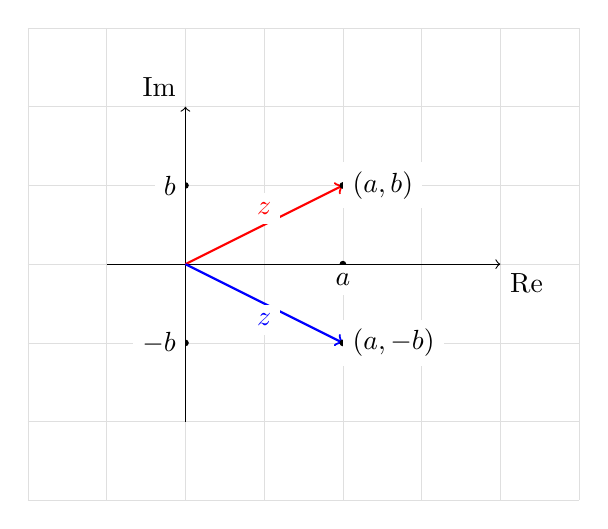
\begin{tikzpicture}
        \draw[step=1cm,gray!25!,very thin] (-2,-3) grid (5,3);
        \draw[thin,->] (-1,0) -- (4,0) node[anchor=north west] {Re};
        \draw[thin,->] (0,-2) -- (0,2) node[anchor=south east] {Im};
        \draw[red,thick,->] (0,0) coordinate (O) -- (2, 1)
        node[midway,above, fill=white] {$z$};
        \draw[blue,thick,->] (0,0) coordinate (O) -- (2, -1)
        node[midway,below, fill=white] {$\conj z$};
        \filldraw [black] (2,0) circle (1pt)
        node[below, fill=white] {$a$};
        \filldraw [black] (0,1) circle (1pt)
        node[left, fill=white] {$b$};
        \filldraw [black] (0,-1) circle (1pt)
        node[left, fill=white] {$-b$};
        \filldraw [black] (2,1) circle (1pt)
        node[right, fill=white] {$(a, b)$};
        \filldraw [black] (2,-1) circle (1pt)
        node[right, fill=white] {$(a, -b)$};
    \end{tikzpicture}
\end{center}

L'operazione di coniugio si comporta bene rispetto alla somma e al prodotto. Vale infatti la seguente proposizione.

\begin{proposition}\label{somma_prodotto_tra_coniugati}
    Siano $z, w \in \C$ tali che $z = a+ib$, $w = c + id$ (con $a, b, c, d \in \R$). Valgono le seguenti affermazioni.
     \begin{enumerate}[label={(\roman*)}]
        \item La somma dei coniugati è il coniugato della somma: \[
            \conj{z} + \conj{w} = \conj{z + w}.
        \]
        \item Il prodoto dei coniugati è il coniugato del prodoto: \[
            \conj{z}\cdot\conj{w} = \conj{zw}.
        \]
        \item $(\conj{z})^n = \conj{z^n}$.
    \end{enumerate}
\end{proposition}
\begin{proof}
    Dimostriamo i tre fatti separatamente.
    \begin{enumerate}[label={(\roman*)}]
        \item Per definizione di somma \begin{alignat*}
            {1}
            \conj{z} + \conj{w} &= (a-ib) + (c - id)\\
            &= (a+c) - i(b+d)\\
            &= \conj{z + w}.
        \end{alignat*}
        \item Per definizione di prodotto \begin{alignat*}
            {1}
            \conj{z}\cdot\conj{w} &= (a-ib)(c - id)\\
            &= (ac - bd) + i(-ad-bc)\\
            &= (ac - bd) - i(ad+bc)\\
            &= \conj{zw}.
        \end{alignat*}
        \item Dimostriamolo per induzione su $n$.
        \begin{description}
            \item[Caso base.] Se $n = 1$ allora banalmente $(\conj{z})^1 = \conj{z} = \conj{z^1}$.
            \item[Passo induttivo.] Supponiamo che la tesi valga per $n$ e dimostriamola per $n+1$. Allora \[
                (\conj{z})^{n+1} = (\conj{z})^{n} \cdot \conj{z} = \conj{z^n} \cdot \conj{z} = \conj{z^{n+1}}
            \] dove l'ultimo passaggio è giustificato dal punto precedente della dimostrazione. \qedhere
        \end{description}
    \end{enumerate}
\end{proof}

Possiamo studiare inoltre le relazioni che un numero complesso ha con il suo coniugato.

\begin{proposition}\label{somma_prodotto_col_coniugato}
    Sia $z = a+ib \in \C$ (con $a, b \in \R$). Allora valgono i seguenti fatti:
    \begin{enumerate}[label={(\roman*)}]
        \item La somma di un $z$ con il proprio coniugato è un numero reale, ed in particolare è il doppio della parte reale di $z$: \[
            z + \conj{z} = 2\Re{z}.
        \]
        \item Il prodotto di $z$ con il suo coniugato è un numero reale, ed in particolare è il modulo di $z$ al quadrato: \[
            z\conj{z} = \abs{z}^2.
        \]
    \end{enumerate}
\end{proposition}
\begin{proof}
    Dimostriamo i due fatti.
    \begin{enumerate}[label={(\roman*)}]
        \item Per definizione di somma vale che \[
           z + \conj{z} = (a + ib) + (a - ib) = 2a = 2\Re z.   
        \]
        \item Per definizione di prodotto vale che \begin{align*}
            z\conj{z} &= (a + ib)(a - ib)\\ 
            &= (a^2 - (-b^2)) + i(ab - ab) \\
            &= a^2 + b^2 \\
            &= \abs{z}^2. \qedhere
        \end{align*} 
    \end{enumerate}
\end{proof}

Dalla seconda relazione della proposizione precendente possiamo ricavare il reciproco del numero complesso $z = a+ib$:
\begin{equation}
    z \cdot \conj z = \abs*{z}^2 
    \iff \frac{1}{z} = \frac{\conj z}{\abs*{z}^2} = \frac{a}{a^2 + b^2} - i\frac{b}{a^2 + b^2} \in \C.
\end{equation}

Dunque ogni numero complesso diverso da $0 + i0$ (in quanto $\abs*{0}^2 = 0$) ha un inverso, calcolabile con la formula di sopra. L'insieme dei numeri complessi con le operazioni di somma e prodotto è quindi un \emph{campo}: \begin{itemize}
    \item valgono la proprietà commutativa e associativa per entrambe le operazioni;
    \item vale la proprietà distributiva;
    \item esiste un elemento neutro per la somma e ogni numero ammette un opposto;
    \item esiste un elemento neutro per il prodotto e ogni numero non nullo ammette un reciproco.
\end{itemize}

\section{I numeri reali come sottoinsieme dei complessi}

I numeri complessi con parte immaginaria nulla, ovvero della forma \[
    a + i0    
\] possono essere interpretati molto semplicemente come numeri reali veri e propri.
Infatti \begin{itemize}
    \item la somma di $z, w \in \C$ con $\Im z = \Im w = 0$ ha ancora parte immaginaria nulla, e corrisponde alla somma delle parti reali: \[
        z + w = (a + i0) + (b + i0) = (a + b) + i0.    
    \]
    \item il prodotto di $z, w \in \C$ con $\Im z = \Im w = 0$ ha ancora parte immaginaria nulla e corrisponde al prodotto delle parti reali: \[
        zw = (a + i0)(b + i0) = (ab + 0) + i0 = ab + i0.    
    \]
    \item il modulo di $z \in \C$ con $\Im z = 0$ corrisponde al valore assoluto della parte reale: \[
        \abs*{z} = \sqrt{a^2 + 0^2} = \sqrt{a^2} = \abs*{a}.    
    \]
    \item il coniugato di $z \in \C$ con $\Im z = 0$ è $z$ stesso: \[
        \conj z = a - i0 = a + i0 = z.    
    \]
    \item il reciproco di $z \in \C$ con $\Im z = 0$ corrisponde al reciproco della sua parte reale: \[
        \frac1z = \frac{a}{\abs*{z}^2} + i\frac{0}{\abs*{z}^2} = \frac{a}{a^2} + i0 = \frac1a + i0. 
    \]
\end{itemize}

Possiamo quindi identificare i numeri reali con il sottoinsieme dei numeri complessi con parte immaginaria nulla: graficamente, essi corrispondono all'asse delle ascisse.